
\chapter{心智和思维}

\section{心智之间能够彼此映射吗?}

既然我们已经假定了在大脑中存在着层次非常高的活跃子系统(即符号),下面就可以回到两个大脑之间可能有的同构或部分同构这个问题上了。我们不关心神经元层次上的同构(这肯定不存在),也不关心大脑中的基本组成部分之间的同构(这肯定存在,但没告诉我们多少东西),我们关心的是在符号层次上是否可能有大脑之间的同构:这将是个对应关系,不仅把某一大脑中的符号对应到另一大脑中的符号,而且还把触发模式对应到触发模式。这意味着以相应的方式把两个大脑中相应的符号联系起来。这是真正的功能同构——当初我们试图描述所有蝴蝶的不变量时,说的就是这种同构。

从一开始就很清楚,人类的两个成员之间不会有这样的同构。否则,就他们的思维而言,他俩将完全不可区分,因而他俩必须要有完全相同的记忆——这就意味着他们必须过着一模一样的生活。就是孪生的人都没能——哪怕是在很小的程度上——接近这种理想状态。

对一个人自己来说又怎么样呢?当你回顾自己几年前写的东西时,你会认为“糟透了!”并且对过去的你付之一笑。更糟的是,你也许会对你五分钟前写的东西或说的话也这样看。一旦发生这种情况,就说明你没有充分理解刚才的自己。你现在的大脑到刚才的大脑的那个同构是不完善的。那么,同构于别人的情况怎么样呢?以及同构于别的物种……?

这个问题的另一方面是差别很大的伙伴之间出现的交流。请想想当你读法国十五世纪的诗人弗朗索瓦·维雍在监狱里写下的诗句时,你所跨越的障碍。另一个人类成员,在另一个年代,关在监狱里,说着另一种语言……你怎么能希望在译成了汉语之后,你还能从那些表面词句中感受到其背后的涵义呢?然而,的确有丰富的涵义传达出来了。

\begin{figure}
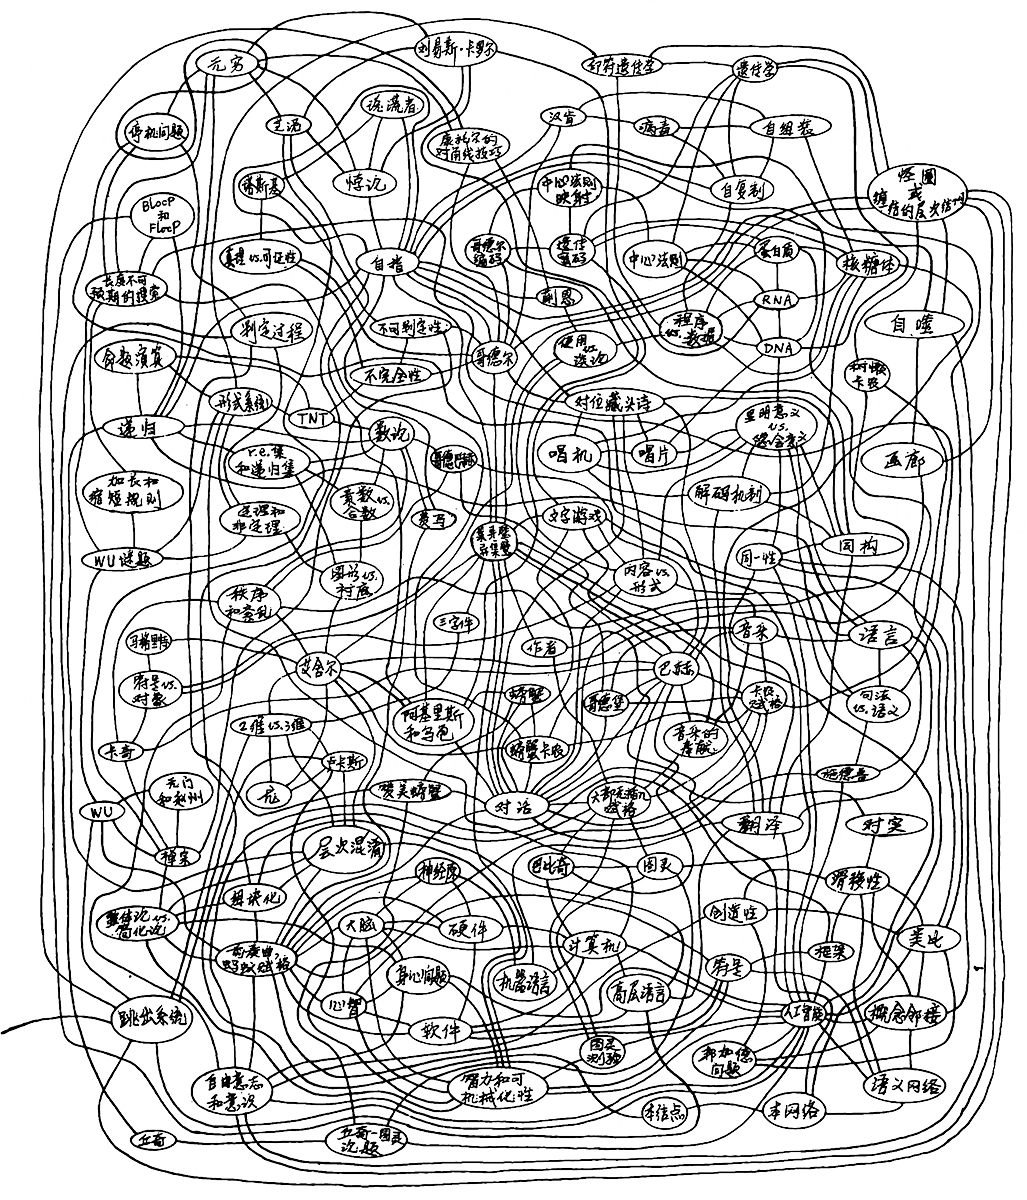
\includegraphics{img_070.png}
\caption[作者的“语义网络”的一个片段。]
  {作者的“语义网络”的一个片段。 }
\end{figure}

因此,一方面,我们可以放弃所有奢望,不再去寻找人们之间精确的同构软件,但是另一方面,很清楚,某些人的思维之间比另一些人的思维之间有更多的类似之处。结论似乎很明显:存在着某种部分的软件同构,将思维风格相似的大脑联系起来——具体说就是,\pnum{1}所有可选符号的对应,\pnum{2}符号的触发模式的对应。

\section{不同语义网络的比较}

但什么是部分同构?这是个很难回答的问题,而且由于下述事实而变得更加困难:没人找到过适当的方法来表示符号的网络及各种符号的触发模式。有时候对这样的符号网络的一小部分可以画出一个图,每个符号在图中表示成一个结点,在每个结点处都引进或引出一些弧线。这些弧线从某种意义上说代表着触发关系。这样的图可以在一定程度上反映我们对概念间的“邻接关系”的直观见解。然而,有各种各样不同的“邻接”,而且在不同的情况下,其作用也各不相同。\fig{70}表示了我自己的“语义网络”的很小一部分。问题是,要想描述许多符号之间复杂的相互依赖关系,只用几条连接顶点的弧线是不太容易做到的。

这种图解的另一个问题是把一个符号简单地看成了“开”或“关”,这是不准确的。虽然对于神经元确实如此,但对于更高一层的神经元集团就不是这样了。在这个问题上,符号比神经元复杂——这你也许料到了,因为它们是由许多神经元组成的。符号之间交换的信息要比仅仅是“我现在被激活了”这一事实更为复杂。后者更像是神经元层次的信息。每个符号可以由许多种不同的方式激活,而激活的类型又影响着它会去激活的那些别的符号。这些缠绕在一起的触发关系怎样用图形的方法表示——真的,它们是否能被表示?——还不清楚。

但是目前,假定这个问题已经解决,假定我们现在承认有那么一种图,上面画着一些由弧线连结起来的结点(其中弧线还是各种颜色的,因而各种类型的概念邻接可以彼此区别开),由此精确地抓住了一个符号触发另一个符号的方式。那么,在什么条件下我们才会觉得两幅这样的图是同构的,或差不多是同构的呢?由于我们处理的是符号网络的图形表示,让我们来考虑一个类似的图形问题。现在有两个蛛网,要确定它们是不是同一种类的蜘蛛结的网,你会怎么做?精确地把各个相应的顶点等同起来,从而建立起一个网到另一个网的精确映射,其中顶点对应顶点,丝线对应丝线,也许甚至连丝线与丝线的夹角也对应起来,你会这样做吗?这必然是无效的努力。两个网永远不会完全相同,然而,还是有某种“风格”、“形式”等等,可靠地标出同一种类的蛛网。

任何网状结构,例如蛛网,都可以考察其局部性质和总体性质。考察局部性质只需要近视的观察者——例如一次只能看到一个顶点的观察者,而考察总体性质只需要大范围视野,不必注意细节。因此,蛛网总的形状是总体性质,而会聚在顶点的平均蛛丝数是局部性质。假定我们同意两个蛛网是“同构”的最合理标准是:它们是由同一种类的蜘蛛做成的。那么一个有趣的问题就是,在断定两个蛛网是否同构时以哪一种观察——局部的还是总体的——作为指南会更可靠一些?现在先不回答这个蛛网问题,我们还是回到两个符号网络的相似性问题——或者说同构问题,如果你愿意。

\section{“炸脖\textcombine{卧龙}”的翻译}

请想想母语是英语、法语、德语、汉语的人。他们都能极好地驾驭各自的母语,而且都喜欢他们自己语言中有双关含义的俏皮话,那么他们的符号网络是在局部层次上还是在总体层次上相似呢?或者,问这类问题本身就没什么意义?如果看看前面刘易斯·卡罗尔著名的“炸脖\textcombine{卧龙}”及其在三种语言中的译文,这个问题就变得具体了。那是一首诗,其中到处都是作者自己发明的词,它们初看上去似乎是没有意义的,但显然并非完全没有意义。每一处都是精心构思的,那些词借助其语音上、书写上的种种特征唤起了其它有意义的字、词或概念。

我选择这个例子,是因为比起普通的文章,它也许能更好地说明在两个不同的网络——在某种层次上分析时是两个极端不同构的网络——当中,试图找出“相同的结点”这样的问题。通常在语言中,翻译的任务要直接得多,因为原先语言中的每个词或短语,在新的语言中一般都可以找到相应的词或短语。对比之下,像“炸脖\textcombine{卧龙}”这样的诗,其中有许多“词”不带有通常的含义,而是纯粹充当邻接符号的激发者。然而,在一种语言中邻接,在另一种语言中也许就是遥远的。

由此,在以汉语为母语的人的大脑中,词“活济济的”大概会在不同程度上激活像“滑济济的”、“活泼的”、“蠕动着的”以及“拥挤着的”一类的符号。那么在说英语的人的大脑中,“slithy”一词有同样的效果吗?对于一个说英语的人,“slithy”会唤起“slimy”[粘糊糊的]、“Slither”[滑动]、“slippery”[滑溜的]、“lithe”[柔软的]以及“sly”[狡猾的]。在汉语和英语的联想之间,这些词当然在某种程度上是有重合的,那么是否能说那两个发明出来的词在说那两种语言的人的大脑中唤起了“相对应的事物”?

把这首诗翻译成法语时,一个有趣的特点是换成了现在时态。保持过去时态会使某些不自然的措辞难以避免,而且,法语中现在时态的味道比过去时态要清新得多。翻译家意识到这会“更恰当”——在某种说不清的然而又有些说服力的意义上——并且做了这个变换。谁能说如实地保持英语时态就更好一些?当然,翻译成汉语时,上述关于时态的许多考虑就变得不必要了,因为在汉语里并没有欧洲语言中那些对时态的区分手段。不过时态也仍然是中文译者必须要考虑的一个重要方面。

把这样的一首诗译成汉语时要注意的一个问题是:在英语中发明一个没有意义的词时,仍可以非常容易地把它念出来,就像真有这么个词一样。由于英语语音上的特点,母语为英语的读者遇见一个陌生的词时仍然能把它念出来,或至少是能“默念”出这个词,因而诗人能相当地肯定那些新造的没有意义的词会有什么样的联想,语音上会有什么样的回声。在汉语里情况就多少不一样了。一个汉字中的语音信息几乎总是不确切的。例如,汉字“㺄”是该念成yú(俞)还是tōu(偷)?而对于生造的字“\textcombine{宓豕}”,恐怕让读者猜出它该念什么就几乎是不可能的了。那么,两种语言之间这些语言学的差异是如何影响着进行翻译时要作出的种种抉择呢?

翻译家的本意大概是想让读者把“㺄”读成tōu,因为对应的英文原文是“toves”。法语和德语的翻译采取的是同样的方针,选用了“toves”和“Toven”。就从英语译成法语或德语而言,保持原文中生造词的语音上的特征大概是较好的翻译策略,因为这三种语言具有无数同源的词,并且语音上有极大的相似性。而汉语无论是语音上还是音调上都和英语相距甚远,这个策略在翻译中还必然是可靠的吗?这是个困难的问题。

汉语和英语之间另一个重要差别是,通常一个汉字中的语义信息要比一个英语词的语义信息多。例如,对于一个英语读者,“toves”和“borogoves”到底是种哺乳动物,还是一种昆虫,抑或是一种爬行动物,这是不甚清楚的。译成汉语时,翻译者就必须从大量可供选用的偏旁、部首中作出抉择,比如“虫”、“犭”以及“鸟”,以便造出个相应的字。结果是,“toves”的中文翻译是“㺄子”,无疑该是种走兽,而“borogoves”译成“鹁\textcombine{若鸟}\textcombine{勾鸟}子”,很清楚是种鸟。假若翻译者选择把“toves”译成“蝓子”,在汉语读者的大脑中激活的联想会是如何的不同呢?把卡罗尔的《阿丽思漫游镜中世界》(“炸脖\textcombine{卧龙}”就选自这本书)继续读下去,我们知道了“toves”是种奇怪的动物,有点像蜥蜴,也有点像獾,还有点像螺丝锥。汉语的常规是一个部首和一个语音成分构成一个汉字,那么对这个翻译问题可能的解决方案就是无穷尽的了。翻译者可以选用像“\textcombine{犭析}\textcombine{犭易}”这样的词,或者“\textcombine{犭累}\textcombine{犭丝}”,等等。但这样的词所唤起的图像也许会过于具体,因而不那么忠实于原文的精神了——原文的本意在于:唤起的想象要足够模糊,以便给读者充分的空间任想象力驰骋。

翻译者借助汉语的字型特点为原文中发明的词造相应的汉字还有其它方法,比如,从书中我们后来知道了“brillig”的意思是“下午四点,你开始煮晚饭的时候”——换句话说,就是临近天黑,但天依然还是全亮着的那个时间。在那首英文的诗中,唤起“light”[亮]和“broiling”[煮]的概念是由于语音上的相似性——词“brillig”和“broiling”以及“brilliant”[灿烂]之间读音上的邻接。在汉语里,类似的效果是来自视觉上的。翻译者用“白”和“灬”这两个成分构造了一个字,多少与“黑”对应上了,同时也联系于“煮”的观念(部首“灬”源自“火”)。

在其它地方,中文翻译也像原文一样借助了语音上的邻接来唤起种种联想。“mimsy”本是要唤起“flimsy”[薄的]和“miserable”[悲惨的]。中文的翻译是“难四儿”——“又难受又细的像‘丝儿’一样”。这种对应是个好的解决方法吗?判断显然是种美学上的判断,不会有确定的答案。这种翻译工作的乐趣也是无穷尽的。

当面临这类例子时,你会认识到精确得无遗漏的翻译是完全不可能的。然而即使是语言翻译这种反常的困难情况,似乎也能获得某种粗略的等价。为什么会是这样呢?读不同译本的人的大脑之间实际上不是不存在同构吗?答案是:在所有这四首诗的读者的大脑之间存在着一种粗略的同构,部分是总体的,部分是局部的。

\section{自想国}

下面我们来做一个地理游戏,我希望这个有趣的游戏会给上述“准同构”带来某种直观。\lnote{(顺便提一句,这游戏有点类似于明斯基在他那篇关于“框架”的文章中发明的地理类比。读者可以在温斯顿的《计算机视觉的心理学》中找到那篇文章。)}设想给了你一本特制的中国地图册,上面标好了所有的自然地理地貌——河流、山脉、湖泊等等——但没有文字。现在,由你来把它变成一本道路地图册,为你不久就要开始的旅行作准备。你要做的是标明各省的边界并填上名称,然后标出所有的城市、乡镇、所有的公路、大车道、乡村小路,所有的公园、林场、风景区、小坝,所有的机场、车站、等等等等……总之要非常细致,使之成为一份详尽的旅行指南。注意,进行这项工作时必须完全靠你自己,不得与别人讨论,不要查询书籍——这一期间你必须打消接触标准地图册的念头。

你可以开始工作了。记住:尽你所能准确地绘制你的地图是会有报偿的——这你不久就会清楚。自然,你会从大城市及主要公路开始,这些你都很熟悉。然后你填得越来越细。当你的知识用尽了,而你又知道那个地方应该还有些城镇、道路的时候,你可以发挥自己的想象力,编造一些城市名称,标上你估计的人口数目。你可以借助自己想象的道路、车站、公园等等再现那个地区的风味。每个地区都这么做,直到填满整个地图。这项工作大概相当艰苦,你要花一番功夫。最终产品是你私人的“带有个人想象的中国版图”——你个人的“自想国”。

比较你的自想国与中国版图,你会发现在你的故乡那个地区,以及那些你曾旅行过的地方或你曾兴趣盎然地察看过地图的地方,两者都非常一致:四川或广东的某个小城镇(比如说那是你的家乡),北京的天安门广场、故宫、颐和园等等,大概都会如实地标在你的自想国版图上。

\section{版图掉换}

现在,一件令人惊异的事情发生了:你的自想国魔术般地成为现实,而且你正好有一个机会去访问这个国家。一个友好的委员会热情地接待了你,并送给你一辆你最喜欢的那种小汽车。委员会主席握着你的手说,“感谢你精心绘制这里的地图,我代表自想国地理学会的全体成员在此向你致以衷心的问候。作为对你辛勤工作的报偿,在我们国家你将享受一次从容不迫的免费旅行。你可以尽情周游古老美好的自想国,去你想去的任何地方,做你想做的任何事情。我们还特地为你准备了一份详细的旅行指南,相信这会对你有所帮助。好,祝你旅途愉快!”——使你惊讶的是,你拿到的不是你所绘制的地图,而是标准的中国道路地图册。

你按计划踏上了行程,开始都还挺顺利,你沿着主要公路到了一个又一个大城市,实际情况都还与地图基本相符。倒也有些个别出入,不过你没太在意。你心情愉快地换了一辆吉普,开始游览自想国辽阔迷人的乡村。这下你可遇着麻烦了,各式各样稀奇古怪的事情接踵而来。当你在青海湖附近刚察县境内的偏僻小路上转来转去的时候,你发现手里的地图册完全失灵了。你向当地居民问路,他们却没听说过你要找的城镇,也不知道你地图上标的那些公路。他们只知道你提及的大城市,即便如此,去那些城市的路线也和你地图上标的不一样。另外,恐怕还会出现这样的怪事:当地居民认为是很大的城市在你的中国地图册上没有。偶尔他们会谈到一个在你的地图上也标着的城市,但在人口上却差了一个数量级,或者方位完全不对。

\section{中心性和普遍性}

自想国与中国版图在某些方面有很大区别,但却仍然是很相似的,这是什么原因呢?这是因为它们的最重要的城市和交通路线能够彼此对应。它们之间的差别表现在诸如旅行时较少经过的线路、小规模的城市等等。注意,这一点既不能由局部同构来刻划,也不能由总体同构来刻划。某些对应确实到了非常局部的层次——例如,在两个北京中,主要大街可能都是长安街,两者也都有天安门广场——然而在两个西藏,大概除了拉萨就再也找不到一个同样的城镇了。所以区别局部与总体在这里不能解决问题,能解决问题的是就经济、通讯、运输等等而言城市的中心性。一个城市在这些方面越是重要,就越能肯定它会在自想国和中国两者中都出现。

在这个地理类比中,有一点是非常关键的:几乎所有的自想国中都有某些确定的、绝对的参照点:北京、上海、广州等等。根据这些你就能确定自己的方位。换句话说,如果来比较我的和你的自想国,我就能利用关于大城市我们之间已有的一致而建立起一些参照点,借此向你说明我这个自想国中较小的城市在什么位置。如果我设想一个从南坪到汶川的旅程,而你不知道这些城镇在哪儿,我就可以指出我们共同都有的一些地方,从而使你明白我说的是什么。如果我谈起一个从武汉到杭州的旅行,这可以沿不同的路线进行,但旅程本身都能实现,这一点在两个国家里是一样的。如果你对我描述从沈尔丹去白长山的旅行,只要你借助附近的大城镇——它们都共同出现在你我的自想国中——说明你的位置,不断地为我定向,我就能勾画出在我看来是在我这个自想国中的一次类似的旅行。尽管在我这里没有叫这个或那个名字的城镇,我还是会相信这样一个旅行是可行的,说不定还很愉快。

我这里的道路和你那里的道路并不完全一样,但是,用我们各自的地图,你我都能从某个地方到达另一个地方。我们能够这样做,是因为那些在现实世界中预先已有的地理事实——山脉、河流等等——那些在我们绘制地图时,对我们各自都有用的事实。没有那些外部特征,我们不可能会有共同的参照点。例如,如果给你一份法国地图,而给我一份德国地图,然后我们都非常详细地把它们填写好,那么将没有办法在这两个虚构的国家中找到“同样的地方”。必须从完全相同的外部条件开始——否则将完全对不上号。

我们这个地理类比已经说得够多了,现在,我们回到大脑之间的同构问题。读者可能很想知道为什么如此强调大脑同构这个问题。两个大脑是同构的,或是准同构的,或者是根本不同构的,这有什么要紧的?回答是,我们有一种直感:虽然别人和我们在一些重要方面有差别,但仍然在某些深入的和重要的方面和我们“相同”——这是我们人类智能的核心。若是能够确定这个不变的核心,然后描绘出什么样的“旁枝”能够添加上去,从而使得我们每个人都成为那个抽象而神秘的所谓“智能”的一个独特体现,那将是很有教益的。

在我们的地理类比中,城市和乡镇类比于符号,而公路则类比于潜在的触发通道。所有的自想国都有一些共同的东西,例如渤海、东海、长江、黄河、洞庭湖、太行山脉,以及许多主要城市和道路,这一事实是类比于这样的现象:我们所有的人,由于外界的种种现实,不得不以相同的方式建立某一类符号及触发通道。这些核心的符号类比于那些大城市,以它们为参照点不会产生歧义(顺便提一下,城市是一个地点,这并不说明大脑中的符号是小得近乎点状的实体。它们不过是在网络中表示成那种样子而已)。

事实上,每个人的符号网络都有一大部分是具有普遍性的。我们简单地把我们大家的共同之处太多地归于理所当然,以至于很难看到我们和别人究竟有多少共同之处。其实,如果设想一下我们同其他类型的东西——例如石头、汽车、餐馆、蚂蚁等等——有多少共同之处,那会是相当费神的,这时我们同随机抽选的一个人之间大量的重叠之处就显得很清楚了。我们见到一个人时,马上注意到的不是那些一般的共同点。因为我们一旦认出对方也是人,那些就是理所当然的了。在这种时候,我们大都是在标准共同点之外发现一些主要的区别,以及事先没料到的额外的共同之处。

偶尔,你也会发现另一个人没有某些知识,而那些知识在你看来是属于标准的、最低限度的核心里的——就像南京从他们的自想国版图上消失了一样。这几乎是不可思议的。比如说,有些人可能不知道大象是什么,或者不知道谁是国家首脑,或者不知道地球是圆的。这些人的符号网络可能和你的符号网络有根本的不同,以至于很难进行富有成效的交流。另一方面,也许这同一个人与你共同具有某种专门知识——例如桥牌方面的专门知识——这样,你们就可以在有限的领域内很好地进行交流。这就像你遇到了一个与你一样从湖北同一个县来的人,因而你们两个的自想国里有一个极小区域高度相符,使你能够非常流利地向他描述怎样从一个地方到另一个地方去。

\section{语言和文化在多大程度上引导思维?}

如果现在回过头来把我们自己的符号网络和英国人的、法国人的以及德国人的符号网络加以比较,那么,尽管母语不同,仍然可以说我们期待他们有标准的核心范畴符号。我们不期待同他们有共同的高度专门化网络,事实上,我们对随机抽选的和我们有同样母语的人也不作这种期待。使用其它语言的人其触发模式和我们自己的会有某些不同,但是那些主要的范畴符号及其之间的主要路线仍然是普遍适用的,因此比较次要的路线可以用它们作参照加以描述。

现在,我们四个人中的每一个人也许又掌握了一些其他三个人的语言。那么,以什么为标准区别“真正流利”和“基本掌握”?首先,流利说汉语的人使用的词汇多数都有一定的使用频率。一个外国人将从字典、小说或课本中学会一些词——这些词可能在某一时期是流行的或较可取的,但现在使用的频率大大减少了——例如,用“内人”而不用“妻子”,用“绍介”而不用“介绍”,等等。尽管这样说话一般仍能传达意思,但由于选择不寻常的词而带有异国调子。

假设一个外国人学会了在正常频率下使用所有的词,这会使他讲话真正流利吗?可能不会。在词汇层次之上还有联想层次,它作为一个整体隶属于文化——包括历史、地理、宗教、童话、文学、技术等等。例如,要能非常流利地说现代希伯来语,你需要精通希伯来语的《圣经》,因为这种语言吸收了大量《圣经》的短语和它们的涵义。这样的联想层次深深地渗入每一种语言。然而在流利的同时仍然有各式各样的变化余地——否则,真正流利说话的人就会是那样一种人:他们的思维是最没有生气的!

尽管应该认识到文化对思维有很深的影响,但却不应过分强调语言在引导思维过程中的作用。例如,可以被我们称作“手套”的两个东西会被说英语的人理解成两种不同类型的物体“Zgloves”[五指分开的手套]和“mittens”[联指手套]。母语是英语的人比我们更多地意识到这种差别——不过要注意,在中国,南方人会比北方人更多地意识到桔子、柑子以及橙子的差别——北方人可能把他们都叫做“桔子”,而引起这种感知差别的不是母语的不同,而是文化(或亚文化)的不同。

至少就考虑核心而言,母语不同的人其符号之间的相互关系有充分的理由非常相似,因为大家都生活在同一个世界上。当你深入到触发模式那些更为细致的方面时,你会发现共同之处就很少了。这很像这样一种情形:让一些从没有在广西住过的人们设计一些自想国,然后对其中广西的某些农村地区进行比较。不过这没什么关系,只要在主要城市和主要线路上有足够的一致,使整个地图上有共同的参照点就行了。

\section{自想国中的旅行和旅行路线}

在整个自想国类比中,对于什么是思维,我用了一个形象化的说法,而一直没有挑明——即,我暗暗地把“思维”与“旅行”相对应。旅行沿途经过的城镇代表被激活的符号。这不是完美的类比,但却是相当有说服力的。这里有个问题:一个想法在人的大脑中重现足够多次以后,它就会逐渐地组块化(凝结)而形成一个单独的概念。这和自想国里非常怪诞的一种事件相对应:经常重复的旅程会以某种奇异的方式变成新的乡镇或城市!如果还要继续使用自想国比喻,记住下面这一点是很重要的:城市不仅代表基本符号(例如,表示“草”、“房子”、“汽车”的那些符号),也代表着由于大脑的组块化能力而产生的符号——诸如那些表示“螃蟹卡农”、“回文斯”或者“自想国”这类深奥概念的符号。

现在,如果认可进行旅行是恰当地对应于思维过程,那么就有下述难题:实际上任何一条路线,从第一个城市到第二个城市,再到第三个,如此下去,都是可行的,只要你记住这些路线都会经过一些中间城市。这对应于符号的任意序列的激活过程:一个接一个,同时允许加入一些额外的符号——那些出现在半途中的符号。也就是说,实质上能按任何期望的次序激活任何一个符号序列。这样一来,大脑似乎就是个不分青红皂白的系统了,它能吸收或产生任何一种思想。但我们都知道并非如此。事实上有一些思想——我们称之为知识或信念——与随意幻想或幽默开心的荒唐念头有着完全不同的作用。我们怎样才能揭示出梦、瞬间即逝的想法、信念以及各种知识之间的异同呢?

\section{可能的、潜在的、反常的通道}

有些通道(这里“通道”既可以看作是自想国里的,也可以看作是大脑中的)是从一个地方到另一个地方的常规路线。还有一些通道必须跟着向导才能走。这种通道称为“潜在的通道”,只有出现特殊的外部环境时我们才走它。那些一次又一次被人们采纳的通道组成了知识——这里我指的不仅是关于事实的知识(描述性知识),也指关于怎样做的知识(过程性知识)。这些稳定可靠的通道构成了知识的内容。各项知识逐渐与信念融合,后者同样由可靠的通道代表,不过大概更容易被替换——比如说,一座桥塌了,或者有大雾的时候。剩下的是幻想、谎言、虚假、谬论以及其它花样,它们对应着一些怪异的路线,比如从北京途径张家口、太原、郑州到济南去。这的确是可能的路线,但大概不是一般的路线——不是人们旅行时通常所采用的路线。

这个模型的一个奇怪而有趣的引申就是,从根本上说,上面列出的各式各样“脱离常轨”的思维完全是由信念及各项知识所组成的。也就是说,任何离奇的、曲折的、间接的通道都可分解为一些不离奇、不曲折、直接的路段,而这些短小的、直接了当的符号连线就代表人们可以信赖的简单思维——信念及各项知识。要是认真想一想,这其实并不令人惊奇。道理很简单:我们能够虚构出来的事情,都是以某种方式根植于我们所体验到的现实中的,不论两者有多大的差异。梦也许就是这种在精神里的自想国的随意漫游。局部地看,它有意义——但是整体上看时……

\section{小说翻译的不同风格}

读一首类似“炸脖\textcombine{卧龙}”的诗,就像在自想国中做一次不切实际的旅行,沿着非常古怪的路线迅速地从一个地方跳到另一个地方。那些译文传达了诗的这一侧面,而不是精确地表示那些触发了的符号序列(尽管对此他们做了最大的努力)。在翻译一般的文章时,这样的跨越并不常见。但这类翻译问题的确是有的。假定你在将一本俄文小说翻译成中文,你碰见一个句子,照字面意思翻译出来就是“她喝了一杯伏特加酒”。现在也许你认为你的读者对于什么是伏特加酒没有概念。你可能会试着用他们的文化中“相应”的词来替代——这样,你可以把它译成:“她喝了一杯茉莉花茶”。如果你认为这个例子是个笨拙的夸张,那么你看看陀斯妥耶夫斯基的小说《罪与罚》的第一句话,先看俄文原文,再看几种不同的中文译文。碰巧这部作品有三种不同的中文译本,其中有不少很有意思的事情。

这第一个句子中出现了街道名字“\textcyr{С-й переулок}”[C胡同]和“\textcyr{К-н чост}”[K桥]。这是什么意思?如果一位细心的陀斯妥耶夫斯基作品的读者,他了解列宁格勒(过去叫“圣彼得堡”——或者应该说是“彼得格勒”?),仔细地核对书中其它地理名称(那些地名也只是给出首字母),就会发现那条胡同必定是“\textcyr{СтолярнЫй переулок}”(斯陀里亚尔尼胡同)。而那座桥的名字不太容易搞清,我们只能知道是个以“K”开头的人名。陀斯妥耶夫斯基大概是想逼真地讲他的故事,但并不想真实到人们能从文字中得知那些地方的地址——在那里,他使得种种罪行及其它事件发生。在任何情况下,都有个翻译上的问题,或者更确切地说,我们在几个不同层次上都有各种翻译上的问题。

首先,我们是否应该保持首字母,使在这本书第一个句子里就出现了的半神秘气氛得以再现?要是这样,我们就应该用“C胡同”和“K桥”。三位译者中只有一个采取了这个方针。这个译本的读者会感觉到原文的“俄国味”,因为那些地方的名字仍然用的是西里尔字母,从而代表着俄文词。

但若是翻译者想保持原作者隐匿真实地名的意图,同时又觉得熟悉西里尔字母的人太少,又会如何?译者可以选用罗马字母,因为中文读者对罗马字母是相当熟悉的,拼音是罗马字母,数学及各门科学的教科书中也大量地用罗马字母表示变量及未知数。这种方针将导致选用“S胡同”和“K桥”——依然是有种很强烈的“外国味”。第二个译者就是这么做的。这也是我高中时读的那部《罪与罚》英译本所采用的方针。我永远不会忘记,当我开始读这篇小说,遇到了那些仅仅由字母作为名称的地方时,我所体验到的迷惑之感。这本书的开头就使我有了某种莫名的不适。我肯定我漏掉了一些本质的东西,然而我不知道那是什么……我断定所有的俄国小说都是离奇的。

第三位译者取了个折中,保持了“S胡同”,但给出了桥的名字:“康桥”。除去这几种办法,我们也可以坦诚地对待读者(可以假定,读者大概对于到底这些地方是真的还是虚构的没有哪怕是一丁点想法!):利用我们的现代学识,写下“斯陀里亚尔尼胡同”。但假若我们再往前走一步,把那地名的意思翻译过来——而非音译——会怎么样呢?“\textcyr{столяр}”的意思是“木匠”,“\textcyr{нЫй}”是个形容词词尾,于是这就可以译成“木匠胡同”。这样,我们就可以设想我们是在北京,不是在彼得格勒,处在老舍虚构的情境中,而不是陀斯妥耶夫斯基的。这是我们想要的吗?也许我们应该干脆换一本老舍的作品来读,并为自己辩护说这是一部“中文中相应的作品”。从足够高的层次上来看,它是陀斯妥耶夫斯基小说的一种“译本”——事实上,是可能有的最好的一个!谁需要陀斯妥耶夫斯基?

我们已经从丝毫不差地忠实作者风格的尝试,一直谈到了保持韵味的高层次翻译。现在如果对第一个句子已经做到了这一点,你能设想在书的其余部分会怎样进行下去吗?当一个德国老板娘操着德国味儿的俄语开始大声喊叫时怎么办?你怎么把带着德国口音说出的断断续续的俄语译成汉语呢?

然后你或许还要考虑俗语及口语表达方式的翻译问题。你是该去找一个“类似”的短语,还是该满足于字对字的翻译?如果你是去找一个类似的短语,那么你就要冒着犯“茉莉花茶”类错误的风险。但如果你字对字地翻译每一个习惯用语,那么你这汉语听起来就会有外国味道。也许这是你所期望的,因为俄国文化对于说汉语的人来说是外国文化。但是一个读这种译本的说汉语的人将由于这种不寻常的词序而不断地体会到一种陌生的——人为的——感觉,不是作者想要表达的,也不是俄文原本的读者所体验到的。

或者换一个问题。设想有这么一本英文书,其中有无数英语中的双关语和文字游戏。有人想把这本书译成中文。书中有幽默的对话,涉及了藏头诗、词首字组合等种种形式与内容上的游戏。译者是否只须字对字把原文译出来,添加无数的脚注,用令人感到折磨的说明文形式来解释原文中那些令人轻松愉快、赏心悦目的机巧?无疑这并不忠实于原文的精神。也许译者应该努力在汉语中重建那些双关机制,在这一过程中改换了许多内容上的细节部分,但保持了原文中的核心内容。进一步来讨论的话,假定这本书中有一段涉及对一本俄文小说在英文中的各种译本进行比较。译者是否应该仅是原原本本把这一段译成汉语,然后加许多脚注来解释那些英语词的意思?或者换一种方式——即重写这个段落,对这本小说在汉语中的几种不同译本进行比较——是不是更好?毕竟,这种选择是旨在用一种易懂并有说服力的方式,提出一些有趣的翻译问题以供讨论,而非让读者皱着眉头费劲地去弄懂一件不是用他们的母语描述的事情。但若是译者走得那么远了,有什么必要还是讨论原来那本俄文小说?海明威的小说或者加缪的小说是不是也行呢?也许也行。什么时候你才离原文的精神实质太远了呢?什么是可以变通的,什么是实质性的?

像这样的问题会使人们联想到有关计算机翻译的种种说法,例如,第一批计算机翻译的提倡者之一——华伦·维佛尔在二十世纪四十年代后期曾提出:“\quotetext{当我看一篇用俄文写的文章时,我就说,‘这实际上是用英文写的,只是用一些奇怪符号进行了编码。我现在要进行解码工作。’}”\note{华伦·维佛尔,“翻译”,载于威廉·洛克和唐纳德·布思[William N. Locke;A. Donald Booth]编的《语言的机器翻译》[\bn{Machine Translation of Languages}],纽约:John Wiley and Sons和马萨诸塞,Cambridge:M. I. T. Press,1955年版,第18页。}维佛尔的话不能仅从字面上理解。相反,它必须被看成是以一种富于启发的方式在说明:有一种可以客观地描述的意义——或至少是某种相当接近客观的东西——隐藏在符号之中。所以,没有理由假定即使有编制得足够好的程序,计算机也无法捕捉到意义。

\section{程序之间的高层次比较}

维佛尔说的是不同的自然语言之间的翻译。现在我们来考虑两种计算机语言之间的翻译问题。比如说,假定有两人分别编写了运行在不同计算机上的两个程序,而我们想知道这两个程序是否执行同样的任务。我们怎样才能知道呢?我必须比较这两个程序。但应该在什么层次上比较?也许一个程序员用机器语言写,另一个程序员用编译语言写。这样的两个程序是可比较的吗?当然可以。可是怎么比呢?方法之一就是编译那个编译语言程序,产生一个该计算机上的机器语言程序。

现在我们有两个机器语言程序。但还有一个问题:这里是两台计算机,因此是两种不同的机器语言——而且可能是极不相同的。一台机器可能是十六位字长,而另一台则可能是三十六位字长。一台机器可能有内部堆栈处理指令(推入与弹出),而另一台没有。两台机器硬件上的差别也许会使这两种机器语言看上去不可比较——而我们依然觉得它们是在执行同样的任务,而且希望一眼就看出这一点。显然,我们现在看这两个程序时离得太近了。

我们需要做的是后退一步,离开机器语言,采用较高层次的、组块化的观点。我们希望从这一有利角度能看出程序中的组块,这些组块使程序看上去是经过了合理的全局——而非局部——设计。也就是说,程序是由这些组块很好的配合在一起而组织成的,使我们能领会程序员的目的。让我们假定这两个程序最初都是用高级语言写的,那么某种组块就已经有了。可是我们会陷入其它麻烦。高级语言的数目在迅速增多:Fortran、Algol、Lisp、APL以及众多其它的语言。你怎么比较用APL写的程序与用Algol写的程序?当然不能是一行一行地比。你将再次在心里对这些程序进行组块,寻找能彼比对应的概念功能单位。所以,你不是在比较硬件,也不是在比较软件——你是在比较“以太件”——那些在软件背后的纯粹概念。在你能实行任何一种有意义的比较之前,你必须从低层次中拔出某种抽象的“概念骨架”,不论你是在比较用两种不同的计算机语言写成的程序,还是比较两种动物,或者是比较两种不同的自然语言写成的句子。

这就把我们带回到一个以前提出来的问题上,那是关于计算机与大脑的:我们怎样才能理解计算机或大脑的一个低层次描述?在这么复杂的系统里,有没有一种从随便什么合理意义上说都是客观的方法,可以从低层描述中抽出高层描述?在计算机的情形中,完全展示存储器的内容——这称为存储器转储——是容易做到的。用计算机进行计算的早期年代里,程序出错时通常都打印出全部存储器内容。然后程序员就不得不回家去,花几个小时钻研存储器的内容,努力去理解存储器的每个小片断都表示了什么。实质上,这个程序员要做的工作与一个编译程序所做的工作正好相反:他要把机器语言翻译成高层次语言,一种概念级别上的语言。结果,这个程序员理解了这个程序的目标,并能用高层次的语汇来描述——例如,“这个程序把英文小说翻译成中文”,或者“这个程序根据输入的任何主题写出八声部赋格曲”。

\section{大脑之间的高层次比较}

现在我们该从大脑的角度来研究上述问题了。这时问题是这样提出的:“人的大脑也能在高层次上被‘读出’吗?有没有对大脑内容的客观描述?”在《蚂蚁赋格》中,食蚁兽宣称,他能通过察看奔忙的蚁群——蚂蚁的组成部分——而得知蚂蚁在想什么。会不会有什么超人——也许,是个“食神经元兽”——存在,可以想象他俯视我们的神经元,把所看到的进行组块,得出对我们思维的分析?

当然,回答必须是肯定的,因为我们在任何时候都能用关于组块的词语(即:非神经元的)去描述我们的意识活动。就是说我们有一种机制,使得我们能够对我们的大脑状态进行粗略的组块,并对之进行功能描述。更确切地说,我们并不对所有的大脑状态都进行组块——我们只是对活跃部分进行组块。然而,如果别人就某一问题向我们提问,而那个问题编码在我们大脑中当前不活跃的区域里,那么我们几乎能在瞬间里进入那个休眠区域,并对那个问题给出组块化的描述——就是说,给出关于那个问题的信念。注意,我们的描述中没有任何关于大脑中那一部分的神经元层次上的信息:我们的描述是高度组块化的,以至于我们甚至一点都不清楚我们描述的是大脑中的哪一部分。这恰好和那个程序员的例子成为鲜明对照:他的组块化描述来自对存储器全部内容的每个部分进行有意识的分析。

如果一个人能对自己大脑中的任何部分做出组块化描述,那么一个局外人,掌握了进入那个大脑的一些非破坏性手段,为什么不能做同样的事情呢?那局外人应该不仅能对那个大脑的有限部分进行组块,而且实际上还能给出那个大脑的完整的组块化描述——换句话说就是,完整地列出一个其大脑是可达的人的全部信念。显然这样的描述会有天文数字的规模,不过在这里没关系。我们感兴趣的是,原则上是否存在关于大脑的一个界说良好的、高层次的描述?或者反过来,是否神经元层次的描述——或者某种同样是生理上的、但在直观上还不清楚的什么描述——是原则上存在的描述中最好的一个?毫无疑问,如果我们要探究我们是否能了解自己,那对这个问题的回答将是至关重要的。

\section{潜在信念,潜在符号}

有可能进行组块化描述,这是我的论点。但有了这个描述后,并不是一切就突然清楚明白了。问题是,为了从大脑状态中抽出组块化描述,我们需要一种语言来描述我们发现的东西。看起来,描述大脑的最恰当方式是枚举它能具有的各个种类的思想,以及它不可能具有的种种思想——或者也许是,枚举它相信的事情及它不相信的事情。如果这是我们进行组块化描述时的奋斗目标,那就很容易看出我们将碰上什么样的麻烦了。

假设你想枚举出在一个自想国里能进行的所有旅行。这会有无穷多种可能。可是你怎么确定哪种可能是似乎合理的?而且,“似乎合理”是什么意思?在试图找出什么是大脑中符号到符号的“可能通道”时,我们要碰到的恰恰就是这种困难。我们可以设想四脚朝天的一条狗从空中飞过,嘴里还叼着一根雪茄——或者公路上两个巨大的油煎鸡蛋撞上了——或任何其他的荒唐情景,要多少有多少。我们大脑中可以采纳的不自然的通道,其数目是没有限制的,就像在自想国里能计划无数条不切实际的旅行路线一样。但对于一个给定的自想国,到底是什么构成了一条“合情合理”的旅行路线?而对于一个给定的大脑状态,到底是什么构成了一个“合理”的想法?大脑状态自身是不禁止任何路径的,因为对于任何一条通道,都会有一些环境使之被采纳。大脑的物理状况所提供的信息——如果是正确读出的——不是说明哪条通道可被采纳,而是沿这条通道走时会遇到多少阻力。

在一个自想国里,可以沿着两条或更多的可选择合理路线进行旅行。比如说,从北京到广州的旅行既可以沿东面路线走,也可以沿西面路线走。两者都是合理的。但在不同的情况下人们有各自的倾向。你在这个时候看了地图,并不能得知在遥远的将来的某个时候哪条路线更为可取——那取决于进行旅行时的外界环境。同样,“读出”一个大脑状态将会揭示出,对于给定的一个符号集合,往往有不止一条合理的可选通道能用来连接符号。不过,这些符号之间的旅行未必是要马上发生的,可以只是所读出的大脑状态中的亿万个“潜在的”旅行当中的某一个。由此得出一个重要结论:大脑状态本身不具有说明哪条路线将被采纳的信息。外界环境在决定路线的选择时扮演着极为重要的角色。

这意味着什么?这意味着在不同的环境下,同一个大脑中可以产生出彼此冲突的想法。任何有价值的高层次大脑状态读出形式都必须包括对所有这类彼此抵触的想法的刻画。实际上这是显而易见的——我们全都是一大堆矛盾的混合体,为了把他们统一起来,我们总是在一个特定时刻只表现出其中的一个方面。选择什么是无法预料的,因为事先并不知道什么条件会对选择施加影响。大脑状态所能提供的是——如果恰当地读它——对路线选择的一个有条件的描述。

我们来考察一个例子,看看《前奏曲》中描写的螃蟹的境况。他对奏出乐曲有各种各样的反应。有时候他几乎无动于衷,因为他太了解那支曲子了。另一些时候,他会相当激动,但这样的反应需要外界恰当的触发——比如说,有一位热心的听众在场,对于这位听众来说作品是新的。高层次地读出螃蟹的大脑状态大概就会揭示出那些潜在的激动(以及会导致激动的条件),也会揭示出潜在的麻木(以及会导致麻木的条件)。然而,大脑状态本身不会说出下一次听这支曲子时会出现什么状况。它只能说:“如果有了这样那样的条件,那么就会导致激动;否则……”。

所以,一个对大脑状态的组块化描述将给出一个目录,列出依环境而有条件地引发的信念。由于不可能枚举所有可能的环境,我们只好满足于列出那些我们认为是“合理”的信念。更进一步,我们还不得不满足于对环境本身的组块化描述,因为显然不可能——也不应该——降到原子层次上去刻划环境。因此,我们不可能做出精确的、决定论的预言,指出在给定的组块化环境下,从大脑状态中会抽出什么信念。概括地说就是:一个大脑状态的组块化描述将由一个带或然性的登记表构成,其中列着一些信念(或符号),它们在各式各样“多半合理的”环境中——这些环境本身也是在组块层次上描述的——最可能被唤起(或触发)。脱离背景环境而试图对一个人的信念进行组块是愚蠢的,这恰恰就像不涉及配偶而试图描述一个人“潜在后代”的分布一样。

同样类型的问题也出现在枚举一个给定人脑中所有符号的时候。一个大脑中不仅潜在地有无穷多的通道,还有无穷多的符号。就像前面已经指出来的,新概念总能从已有概念中形成,而且可以争辩说表示这种新概念的符号不过就是潜存在每个个体中等待着被唤醒的休眠符号。它们也许在这个人的一生中从未被唤醒,但却可以宣称那些符号一直是存在于那里的,只等着恰当的环境来触发它们的合成。不过,如果这种可能性非常小,似乎把“休眠”用于这种情况就不太符合实际了。为了使这一点更为清楚,可以试图去想象当你醒着的时候蛰居在你头颅里的所有“休眠的梦”。是否有可能存在一个判定过程,在给定你的大脑状态时能区分开“不可梦想的主题”与“潜在地可梦想的主题”?

\section{自我意识在哪里?}

回顾我们讨论过的问题,你也许会自言自语,“这些关于大脑和心智的思考都挺好,但是涉及到意识的那些知觉怎么样呢?这些符号尽可以随心所欲地相互触发,但除非某个人觉察整个这件事,否则就没有意识”。

直观上这在某个层次上有道理,但在逻辑上却不太说得通。因为这样一来就会迫使我们去寻找一种解释这种机制(觉察所有活跃符号的机制)的说法,如果这种说法还没有包括在我们至今所给出过的描述里。当然,一位“唯灵论者”不必看得这么远——他只需断言所有这些神经活动的觉察者就是灵魂,而灵魂是不能用物理词汇描述的,那就够了。不过,我们将试图给出一个“非唯灵论者”的解释,说明意识出现在哪里。

我们这个有别于“唯灵论者”的解释——这也是个令人困惑的解释——是停在符号层次上说:“这就是它——这就是所谓的意识。意识是系统的一种性质,每当系统中有服从触发模式——多少有点像前几节描述过的触发模式——的符号时,这种性质就会出现”。这么简单,似乎太不够了。这怎么能说明关于“我”的知觉,即自我意识呢?

\section{子系统}

没有理由期望“我”,或者“自我”,不该由一个符号所表示。事实上,表示自我的符号可能是大脑的所有符号中最复杂的一个。出于这个原因,我愿意把它放在分层结构中的一个新层次上,并称之为子系统,而不称符号。确切地说,所谓“子系统”,我指的是符号的集群,其中的每个符号都能在子系统本身的控制下被激活。我想传达出来的子系统图像是这样的:它起的作用几乎像个独立的“子脑”,具有自己的可选符号集,而那些符号则可以在它内部相互触发。当然,子系统和“外界”——也就是大脑的其余部分——也有大量通讯。“子系统”不过是一个生长过度的符号的别称,这种符号已变得非常复杂,其中有许多子符号彼此相互作用。所以,在符号与子系统之间没有严格的层次区别。

由于子系统与大脑的其余部分有广泛的联系(不久就会描述几种这样的联系),所以很难在子系统和外界之间划出明确的界线。但即使边界模糊,子系统仍然是相当实在的东西。有趣的是,子系统一旦被激活,然后撒手不管,它就会自己一直工作下去。这样,一个个体的大脑中两个或更多的子系统可能会同时运转。我就注意到过偶尔发生在我自己大脑中的这类事:有时我发觉我的脑海里响起两支不同的曲子,争夺着“我的”注意力。每一支曲子都是在我大脑中的一个单独隔间里以某种方式制造或“演奏”出来的。两个负责从我的大脑中提取出曲子的子系统大概都各自激活了一系列符号,一个接着一个,完全不顾另一个子系统也在做同样的事情。然后两者都试图同我大脑的第三个子系统——我的自我符号——进行通讯,就在这个时候我大脑中的“我”察觉到发生了什么。换句话说,“我”开始获得了一个关于“那两个子系统的活动”的组块化描述。

\section{子系统和共用编码}

典型的子系统大概是那些代表我们亲密朋友的子系统。那些人在我们的大脑中被表示得非常复杂,以至于代表他们的那些符号扩张到了子系统的级别,变得能自主地活动并且还可以利用我们大脑中的一些资源来维持自己。在这里我的意思是,一个将朋友符号化的子系统能像我自己一样在我的大脑里激活很多符号。比如,我可以启动我的一个代表某好朋友的符号,然后就几乎真的感觉到自己处于他的地位上,冒出他会有的种种想法,激活那些更多地是反映他的思维模式的符号序列。可以说我这个朋友的模型——在我大脑中体现为一个子系统——就构成了我对他大脑的一个组块化描述。

那么,对于那些我认为在他大脑中会有的符号,这个子系统是否包括了一些与之分别对应的符号呢?这其实是多余的,很可能这个子系统会大量利用我大脑中已有的符号。例如,当我大脑中表示“山”的那个符号被激活时,它就可以被这个子系统借去。这时,子系统使用那个符号的方式不必等同于我整个大脑使用它的方式。具体说,如果我在和我的朋友谈论亚洲中部的天山山脉(我们俩都没去过),并且我知道几年前他在阿尔卑斯山有过一段极棒的远足经历,那么我心里对他的那些谈论的解释就会部分地带有我印象中他从前那次阿尔卑斯山经历的色彩,因为我会去努力设想他会如何想象那个地方。

使用我们在本章建立起来的词汇,我们可以说,符号“山”在我这里的激活是受控于我的那个代表他的子系统。其效果是在我的记忆中打开一个通常情况下我不用的窗口——就是说,我的“缺席选择开关”从我通常的记忆范围扳向了我对他的记忆的记忆。当然,我对于他的记忆的表示只是他的实际记忆的一个近似,构成他记忆的那些大脑符号彼此激活的形态十分复杂,我是无法全部了解的。

他的记忆在我这里的表示也是处于复杂的大脑符号彼此激活的形态,当然这里是我的大脑中的符号——即那些“原始的”概念,例如草、树、雪、天、云等等。我必须假定在他那里对这些概念的表示与在我这里是“等同的”。我还必须假定对更基本的观念我们俩也有类似的表示,如重量、呼吸、疲劳、颜色等感觉。登上峰顶瞭望四周景色时的愉悦感虽不那么基本,却也几乎是每个人都会有的。

因此,我的大脑中产生这种愉悦感的复杂机制可以直接搬到“朋友子系统”中去,而且不会太走样。

我们可以接着做下去,尝试去描绘我怎样完整不漏地理解朋友讲给我的一个故事,一个充满了复杂的人际关系和心灵体验的故事。可是我们的术语很快就会变得不够用了。当涉及对这个或那个事情的他所表示的我所表示的他的表示时,就会现出复杂的递归。假如故事中还有我们共同的朋友,那么我会在我自己关于他们的形象和我关于他那里对他们形象的表示之间寻找调和。纯粹递归在处理这种类型的符号混合物时显然是种不适用的形式手段。况且我们只不过才触及到问题的表面!我们目前实在缺乏词汇去描述符号之间可能有的复杂的相互作用。所以在我们陷入窘境之前还是止步为好。

不过我们应该注意,计算机系统在某些方面已经开始达到同样类型的复杂性,而这些概念中的一部分也因此有了名称。例如,我的“山”符号就类似于计算机术语中的共用(可重入)编码——那些可同时被运行在一台计算机上的两个或更多的分时程序使用的编码。当一个符号同时是几个不同子系统的部分时,激活它就会有不同的结果。这一事实可以作这样的解释:那个符号的编码在被不同的解释程序处理。所以,“山”符号中的触发模式不是绝对的,而是和在哪个系统中激活符号有关。

有些人可能会怀疑这种“子脑”的真实性,下面是艾舍尔在谈论他怎样创作他那些充溢在平面里的循环画时说的一段话,也许对弄清我这里指的是什么现象会有所帮助:

\begin{quote}
当我作画时,有时会觉得似乎自己是个巫师,被我召唤出来的灵物所控制。好像是它们在决定选择什么形状来显现自己。它们在诞生过程中,一点也不考虑我的评判,它们将怎样发展我也施加不了多少影响。它们通常都是些很难对付并且很固执的家伙。\note{麦克吉拉弗里,《艾舍尔周期循环式绘画的对称问题》,第VIII页。}
\end{quote}

这是个理想的例子,说明大脑中某类子系统一旦被激活,就几乎是自主的了。对于艾舍尔来说,他的子系统几乎能统治他的审美判断力。当然,不能把这一点看得太绝对,因为那些强有力的子系统是作为一个结果,来自他多年的训练并严格服从那种塑造了他的审美意识的力量。总之,如果把艾舍尔大脑中的那些子系统与艾舍尔本人或他的审美判断力分隔开,那就错了。在他的美感中,“他”是这个艺术家的完整自我,而那些子系统是必不可少的组成部分。

\section{自我符号与意识}

自我子系统活动时有一个非常重要的旁效,即它在下述意义上能扮演“灵魂”的角色:在不断地与大脑中其他子系统及符号进行通讯时,它密切注意着哪个符号处于激活状态,以及是以什么方式在活动。这就是说它必定有表示心智活动的符号——换一种说法,就是那些表示符号的符号,以及表示符号活动的符号。

当然,这并没有把意识或感知提高到什么“有魔力的”非物理的层次上。这里感知是我们所描述过的那些复杂的硬件软件的一个直接后效。这种方式描述感知——即把感知作为大脑本身的一个子系统对大脑活动的监控——尽管源于世俗,仍然和我们都知道并称为“意识”的那种近乎不可描述的感觉相像。读者肯定能看出这里的复杂程度已经足以产生许多意外的效果。例如,很可能一台具有这种结构的计算机会谈论自己,那些话极像人们通常谈论自己时说的,包括固执地强调它有自由意志,它不能被解释成“部分的总和”等等。(有关这方面的问题,可参阅明斯基的文章《物质、心智和模型》)。

我一直假定有一个表示自我的子系统。怎么能保证这样的子系统实际存在于我们的大脑里呢?如果没有自我符号的发展演化,一整套复杂的符号网络——比如我们上面描述过的那种——也能够发展演化吗?如果没有一个表示宿主有机体的符号,这些符号及其活动怎么能实现那些“同构”于周围世界中的实际事件的心理事件呢?进入系统的所有刺激在片刻中都集中在一个很小的空间范围之中。要是没有一个表示有机体的符号,处于这个有机体中的大脑符号结构就会有一个很显眼的洞,需知,在这个大脑符号结构所反映的事件中,那个有机体扮演着一个比其它对象都更重要的角色。事实上,仔细想一想的话,理解那个围绕着一个生物体的世界的唯一途径,似乎就是在与周围物体的关系中理解这个生物体所起的作用。这就必须要有一个自我符号存在。而且,从符号到子系统这一步骤也不过是反映了自我符号的重要性,并非质的变化。

\section{我们与卢卡斯的初次会面}

牛津哲学家卢卡斯(和我们前面谈到的“卢卡斯数”没有关系)于1961年写过一篇引人注目的文章,题目是“心智、机器和哥德尔”。他的观点和我的观点几乎完全对立,然而他用来论证他的观点的材料中有许多和我的材料相同。下面这段节录与我们刚才的讨论有很大关系:

\begin{quote}
当一个人第一次进行最简单的哲学探讨时,他就会陷入下面一系列问题:如果某人知道了一件事,他是否知道他知道这件事?一个人自我反思的时候他在想什么,当时是什么机制在进行思维?经过长时间的困惑与挫折之后,他学会了不去纠缠这些问题:他暗暗体会到有意识物与无意识物的概念是不同的。当我们说一个有意识物知道什么事情的时候,我们说的不仅是他知道那件事,还包括他知道他知道那件事,以及他知道他知道他知道那件事,如此下去,直到我们不再纠缠这个问题——在这里我们识别出了无穷,但并不是什么不好意义下的无穷回归,因为逐渐消失掉的并不是答案,而是那个没多少意义的问题。感到这些问题没有意义,是因为在其概念自身中包含着对这些问题的回答能无限进行下去的思想。

虽然有意识物有能力进行下去,我们不希望仅仅作为一系列他们能从事的工作而展示这一点,也不把心智看作是一个自我和超自我和超超自我的无穷序列。相反,我们坚持这样的观点:有意识物是个整体,虽然我们也谈论心智的各个部分,但那只是一种比喻的说法,不能按字面意义理解。

意识悖论的出现是因为有意识物除了能意识到别的东西,还能意识到自身,并且的确不能看作是可分解的。这意味着有意识物可以用某种手段处理哥德尔式的问题,而机器却不能用同样手段。这是因为有意识物可以既考虑自己也考虑其工作,同时依然是在那里进行工作,而不是在干别的。一台机器可以被制造成那种所谓能“考虑”它在干什么的机器,但它无法在工作时把它的所作所为“考虑进去”,除非它变成一台新的机器,也就是说,这台机器加上了一个“新的部分”。但在我们关于有意识的心智的观念中,能反思自己和评判自己的所做所为是它固有的特点,不需要外加的部分:它已经是完备的了,没有固有的致命弱点。

这样,我们的论题开始变成更多地是属于概念分析问题,而非数学发现。这一点由图灵提出的另一个论据所证实。至今,我们只造出了相当简单的并且是可预知其行为的人工制品。随着我们增加机器的复杂度,也许会有令人惊讶的事情在等着我们。他用核反应堆的裂变作比较。在某个“临界点”之下,几乎没什么事情发生,但是一旦超过临界点,就会火花四溅。大脑和机器或也许是这样。多数大脑和所有的机器目前都是在“临界点”之下的——它们对受到的剌激冷漠而迟钝,而且毫无主见,只能作出平庸的反应——但现在有少数大脑,以及将来可能有的一些机器,是超临界点的,能独自焕发出光彩。图灵的意思是,这只是个复杂程度问题,超过某种复杂水平就会出现质的变化。因此“超临界”的机器会与人们迄今设想的简单机器非常不同。

也许是这样。复杂程度的确经常引起质的不同。尽管听起来难以置信,结果可能就是:在某种复杂度级别之上,一台机器甚至从本质上都不再是可预知的,它开始自行其是,或者换一种富于启发性的说法,就是,当它不再是完全可预知和完全可驾驭时,它也许就开始有它自己的心智了,它能做出一些我们承认是需要智能的事情,而非仅仅是出错或随便瞎猜,同时那还不是我们事先编好程序的。但若是这样,就那些行为所处的背景而言,它已不再是台机器了。在机械论者的争辩中,关系重大的不是心智怎样形成,或心智可能会怎样形成,而是心智怎样活动。对于机械论者的论点来说,关键是心智的机械模型将按照“机械原则”运转,也就是说,我们可以从各个部分的运转去理解整体的运转,而每个部分的运转或者取决于它的初始状态和机器的结构,或者是在一定数目的确定的运转之间作一个随机选择。如果机械论者造出了一台机器,复杂得这一切都不能很好地保持下去,那么对于我们现在的讨论而言,它就不再是一台机器了,无论它是怎样建造的。相反,我们应该说是创造了一个心智,和现在人类生育是同一种意义。于是产生新的心智的方式就会有两种:传统的方式——即妇女生小孩——和新的方式,即建造非常非常复杂的系统:比如说电子管和继电器组成的系统。当谈到第二种方式时,我们应该注意强调,虽然创造出来的东西看上去像台机器,但却不是真正的机器,因为它不单是部分的总和。一个人仅仅知道它的构造及其各部分的初始状态,是无法说出它将会做些什么的,甚至无法说出它能力的极限在哪里,因为即使给它一个哥德尔型问题,它也会正确回答。事实上我们应该简单地说,没有被哥德尔问题难倒的系统就不是图灵机,即:在“对哥德尔问题的反应”这一点上,它们不是机器。\note{卢卡斯,“心智、机器和哥德尔”,载阿·罗·安德森编《心智与机器》,第57--59页。}
\end{quote}

在读这段文章时,我不断地被那一连串的话题、引喻、暗指、混淆以及结论弄得不知所措。我们从卡罗尔式的悖论跳到哥德尔再跳到图灵再到人工智能再到整体论和简化论,全都在短短的两页纸上。卢卡斯这套玩意儿唯一的作用就是刺激我们的思想。以下各章里,我们还将回到在这篇奇怪的文章中许多撩人地一掠而过的话题。


